% Q20：按原图复现斜三棱柱的顶点、可见/隐藏棱及 P,M,N 辅助线。
% 投影为示意布局，不表达未给出的长度或角度。
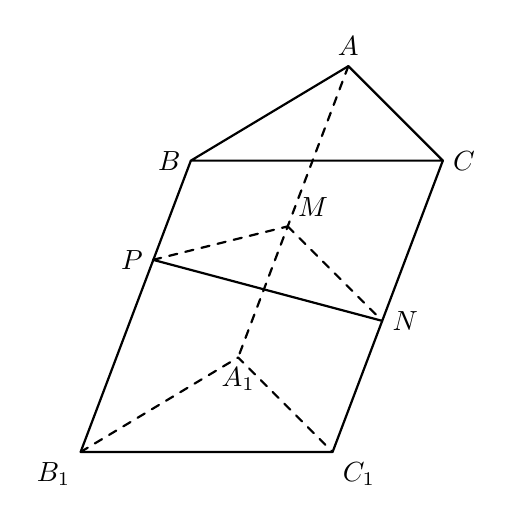
\begin{tikzpicture}[line cap=round,line join=round,thick]
  \coordinate (A)  at (2.0,4.0);
  \coordinate (B)  at (0.0,2.8);
  \coordinate (C)  at (3.2,2.8);
  \coordinate (A1) at (0.6,0.3);
  \coordinate (B1) at (-1.4,-0.9);
  \coordinate (C1) at (1.8,-0.9);
  \coordinate (P)  at (-0.48,1.54);
  \coordinate (M)  at (1.23,1.965);
  \coordinate (N)  at (2.43,0.765);

  % Upper face and visible prism edges.
  \draw (A)--(B)--(C)--(A);
  \draw (B)--(B1) (C)--(C1) (B1)--(C1);

  % Hidden back edge and rear triangular face.
  \draw[dashed] (A)--(A1) (B1)--(A1)--(C1);

  % Auxiliary construction shown in the original.
  \draw[dashed] (P)--(M) (M)--(N);
  \draw (P)--(N);

  \node[above] at (A) {$A$};
  \node[left] at (B) {$B$};
  \node[right] at (C) {$C$};
  \node[below] at (A1) {$A_1$};
  \node[below left] at (B1) {$B_1$};
  \node[below right] at (C1) {$C_1$};
  \node[left] at (P) {$P$};
  \node[above right] at (M) {$M$};
  \node[right] at (N) {$N$};
\end{tikzpicture}
